\chapter{Thiết kế và hiện thực ứng dụng Openlet}
\label{chap:thiet-ke}

Chương này sẽ trình bày kiến trúc và xây dựng ứng dụng Web Openlet nhằm kiểm chứng khả năng ứng dụng vào thực tế của các nghiên cứu trên. Nội dung của chương sẽ bao gồm giới thiệu về ứng dụng, phân tích yêu cầu và trình bày các luồng hoạt động chính để đáp ứng nhu cầu của người dùng cuối.

\section{Giới thiệu ứng dụng và công nghệ sử dụng}

Chương~\ref{chap:phuong-phap} của khóa luận đã trình bày chi tiết các thành phần nghiên cứu cốt lõi của hệ thống Openlet, bao gồm quy trình nhận dạng văn bản từ ảnh, phương pháp sinh câu hỏi trắc nghiệm bằng kiến trúc đa tác tử và khung đánh giá chất lượng của mô hình. Trên cơ sở đó, ứng dụng Openlet được phát triển là một ứng dụng soạn thảo và làm bài kiểm tra trắc nghiệm trực tuyến áp dụng các kỹ thuật đã nghiên cứu trên.

Openlet hướng tới hai nhóm người dùng chính. Nhóm thứ nhất là giáo viên hoặc người biên soạn tài liệu học tập. Đây là nhóm người có nhu cầu lớn trong việc chuyển đổi các tài liệu học tập sang bài kiểm tra trắc nghiệm trực tuyến. Nhóm thứ hai là học sinh hoặc người làm bài. Những người này sẽ truy cập bài kiểm tra qua liên kết chia sẻ, thực hiện làm bài và nhận kết quả phản hồi.

\textbf{Trong phạm vi của khóa luận này, Openlet được thiết kế là một chu trình nghiệp vụ khép kín gồm tiếp nhận tài liệu đầu vào, trích xuất nội dung từ tài liệu, sinh câu hỏi trắc nghiệm, tổ chức làm bài và theo dõi kết quả.} Ứng dụng hỗ trợ ba định dạng tài liệu phổ biến là ảnh chụp tài liệu, tệp PDF và văn bản thuần.

Để hiện thực hóa kiến trúc hệ thống đã đề xuất thành một sản phẩm hoàn chỉnh, việc lựa chọn và kết hợp các nền tảng phát triển phù hợp là yếu tố tiên quyết. Công nghệ được sử dụng để phát triển mã nguồn và triển khai ứng dụng được chia thành ba nhóm chính tương ứng với ba lớp kỹ thuật của hệ thống gồm: Công nghệ phía giao diện người dùng, công nghệ máy chủ và công nghệ trí tuệ nhân tạo.

\textbf{Công nghệ phía giao diện người dùng.} Lớp giao diện của Openlet được xây dựng bằng thư viện \textbf{Next.js} \cite{nextjs} kết hợp với \textbf{React} \cite{reactjs}. Lựa chọn công nghệ này cho phép hệ thống tổ chức giao diện thành các thành phần và trang rõ ràng, thuận tiện cho quá trình phát triển.

\textbf{Công nghệ phía máy chủ.} Để thuận tiện cho quá trình triển khai và vận hành ứng dụng, hệ thống Openlet sử dụng nền tảng \textbf{Firebase} \cite{firebase} làm cơ sở dữ liệu và lưu trữ tệp tĩnh. Ngoài ra, để hệ thống có thể mở rộng linh hoạt, máy chủ được phát triển dưới dạng serverless thông qua tính năng Cloud Functions của Firebase. Cơ chế này giúp hệ thống có thể tách bạch mỗi bước nghiệp vụ trong quy trình thành một hàm thực thi độc lập.

\textbf{Nhóm công nghệ mô hình trí tuệ nhân tạo.} Hệ thống sử dụng các sLLM, VLM và LLM thương mại thông qua API của nền tảng trung gian \textbf{OpenRouter} \cite{openrouter}. Cách triển khai này cho phép hệ thống chuyển đổi linh hoạt giữa nhiều loại mô hình ngôn ngữ khi không có hạ tầng tại chỗ.

\section{Phân tích đặc tả yêu cầu}
\label{sec:phan_tich_yeu_cau}
Trong phần này, khóa luận sẽ tập trung vào các yêu cầu chức năng và phi chức năng mà nền tảng Openlet tập trung phát triển. Trong khi các yêu cầu chức năng tập trung vào các chức năng cốt lõi mà hệ thống phải có để người dùng cuối có thể sử dụng thì yêu cầu phi chức năng tập trung hơn vào trải nghiệm của người dùng và khả năng mở rộng.

\subsection{Yêu cầu chức năng}
\textbf{Hệ thống Openlet được thiết kế và xây dựng xoay quanh hai tác nhân chính là \textit{Giáo viên} và \textit{Học sinh}.} Các yêu cầu chức năng được chia làm hai nhóm tương ứng với hai tác nhân này; Hình~\ref{fig:openlet-use-case} biểu diễn các ca sử dụng của mỗi tác nhân.

\textbf{Giáo viên (Người quản trị bài kiểm tra).} Đây là tác nhân có nhiệm vụ khởi tạo và quản lý toàn bộ quy trình và vòng đời của bài kiểm tra. Các chức năng cốt lõi cần có bao gồm:

\begin{itemize}
    \item \textit{Tạo và quản lý bài kiểm tra:} Tải lên tài liệu đầu vào; lựa chọn cấu hình AI.
    \item \textit{Biên tập nội dung:} Rà soát, chỉnh sửa trực tiếp nội dung câu hỏi, phương án trả lời và lời giải thích do hệ thống sinh ra.
    \item \textit{Cấu hình và công bố:} Thiết lập cấu hình của bài kiểm tra (cho phép ẩn danh, làm lại, thời gian làm bài) và mức độ phản hồi kết quả.
    \item \textit{Theo dõi và thống kê:} Quản lý danh sách các lượt nộp bài của học sinh và xem các chỉ số thống kê tổng hợp (phân bố điểm, bảng xếp hạng thành tích).
\end{itemize}

\textbf{Học sinh (Người làm bài).} Tác nhân này dùng đường dẫn từ giáo viên để làm bài kiểm tra trực tuyến. Các chức năng chính là:

\begin{itemize}
    \item \textit{Truy cập và xác thực:} Truy cập bài kiểm tra qua liên kết chia sẻ; định danh hoặc làm bài ẩn danh tùy cấu hình.
    \item \textit{Thực hiện bài kiểm tra:} Đọc đề thi đã được lọc đáp án, chọn phương án trả lời và nộp bài.
    \item \textit{Nhận phản hồi:} Xem kết quả đánh giá, điểm số và lời giải thích chi tiết theo đúng giới hạn hiển thị của giáo viên.
\end{itemize}

\begin{figure}[htbp]
    \centering
    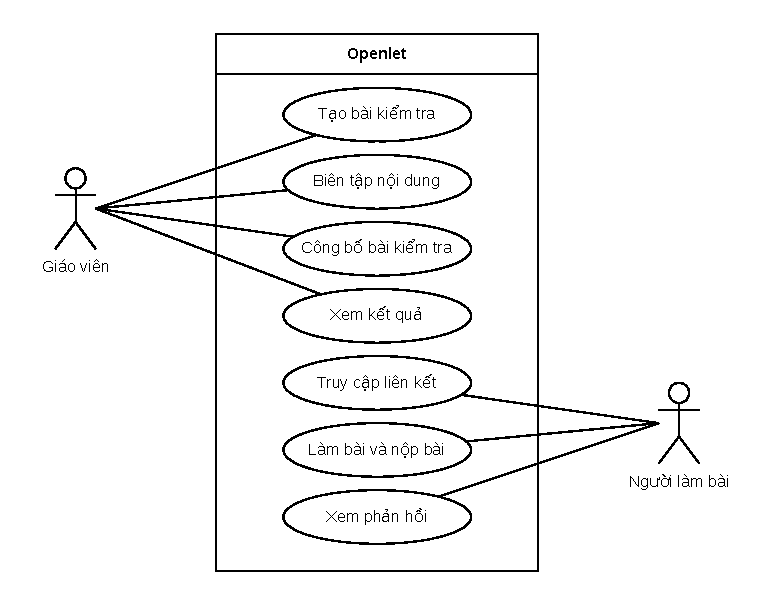
\includegraphics[width=0.8\linewidth]{figures/demo-use-cases.pdf}
    \caption{Biểu đồ ca sử dụng tổng quát của Openlet với hai tác nhân chính: giáo viên (quản lý vòng đời bài kiểm tra) và người làm bài (truy cập và nộp bài)}
    \label{fig:openlet-use-case}
\end{figure}

\subsection{Yêu cầu phi chức năng}

Các yêu cầu phi chức năng quyết định trực tiếp cách kiến trúc hệ thống được thiết kế và triển khai có thể đáp ứng được các yêu cầu này hay không. Do vậy, việc xem xét các yêu cầu phi chức năng của nền tảng cần được triển khai đóng một vai trò quan trọng. Các yêu cầu phi chức năng dưới đây là các yêu cầu có thể được kiểm thử trực tiếp và sẽ được kiểm thử trong quá trình xây dựng và phát triển hệ thống.

\textbf{Tương thích trên nhiều loại thiết bị.} Hệ thống Openlet được xây dựng với triết lý đa nền tảng từ đầu. Giao diện được thiết kế có thể thay đổi linh hoạt dựa vào thiết bị và kích thước màn hình, điều này giúp giáo viên có thể dễ dàng dùng điện thoại chụp hình tài liệu từ dạng vật lý trong khi học sinh có thể sử dụng máy tính để thuận tiện cho quá trình làm bài.

\textbf{Tính mở rộng và linh hoạt.} Máy chủ của hệ thống phải có khả năng hỗ trợ số lượng người dùng đột biến, tự động mở rộng năng lực tính toán của máy chủ. Điều này xuất phát từ đặc điểm cốt lõi của các ứng dụng giáo dục là phải xử lý lượng lớn người dùng cùng lúc khi bắt đầu một bài kiểm tra.

\textbf{Hiệu năng và xử lý bất đồng bộ.} \textbf{Các tác vụ nặng phụ thuộc vào mô hình trí tuệ nhân tạo như OCR và LLM phải được xử lý dưới nền một cách bất đồng bộ mà không gây ảnh hưởng đến các chức năng khác của hệ thống.} Bên cạnh đó, giao diện của người dùng phải được cập nhật trạng thái của tác vụ theo thời gian thực để đảm bảo trải nghiệm người dùng.

\section{Thiết kế hệ thống}
\label{sec:thiet-ke-he-thong}

\subsection{Kiến trúc tổng thể}
Quá trình lựa chọn và thiết kế kiến trúc hệ thống đóng vai trò quan trọng trong việc xác định xem một hệ thống có đáp ứng được các yêu cầu về cả chức năng và phi chức năng hay không. Việc áp dụng một kiến trúc cụ thể không chỉ cần đảm bảo sự thích hợp với yêu cầu hiện tại của hệ thống mà còn phải đề cao khả năng mở rộng và phát triển trong tương lai.

\textbf{Hệ thống Openlet được triển khai theo kiến trúc ba tầng.} Tầng thứ nhất là giao diện Web được cài đặt bằng thư viện \textbf{Next.js} và sử dụng Firebase Authentication để xác thực tài khoản thông qua Google. Tầng tiếp theo là các khối Cloud Functions đóng vai trò xử lý từng công việc nghiệp vụ như chấm điểm, truy xuất đề thi, OCR. Tầng thứ ba là dịch vụ trung gian OpenRouter cung cấp API của các mô hình trí tuệ nhân tạo. Kiến trúc của hệ thống được biểu diễn trong Hình~\ref{fig:openlet-architecture}.

\begin{figure}[htbp]
    \centering
    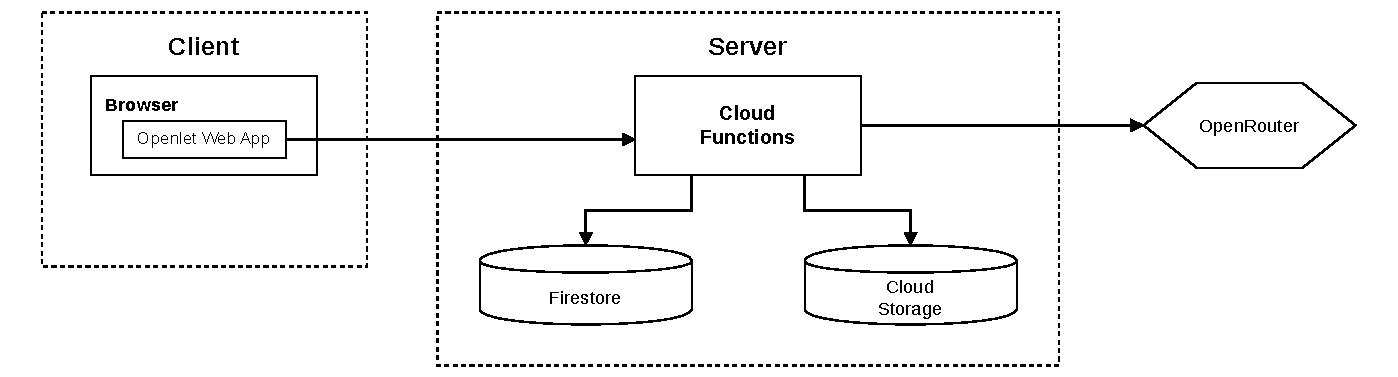
\includegraphics[width=0.95\linewidth]{figures/demo-architecture.pdf}
    \caption{Kiến trúc ba tầng của Openlet: tầng giao diện (Next.js/React), tầng dịch vụ (Firebase), và tầng AI (OpenRouter kết nối các mô hình OCR/LLM)}
    \label{fig:openlet-architecture}
\end{figure}

Các Cloud Functions cốt lõi của hệ thống được tách theo từng bước nghiệp vụ quan trọng nhằm đảm bảo khả năng xử lý bất đồng bộ, bảo vệ dữ liệu nhạy cảm và hỗ trợ mở rộng độc lập theo tải thực tế. Bảng~\ref{tab:cloud-functions} mô tả vai trò của các hàm chính trong luồng vận hành của Openlet.

\begin{table}[htbp]
\centering
\begin{tabular}{lp{0.68\linewidth}}
\toprule
\textbf{Cloud Function} & \textbf{Mô tả} \\
\midrule
\texttt{processDocument} & Nhận ảnh hoặc PDF từ Cloud Storage, gọi mô hình OCR và cập nhật văn bản trích xuất vào Firestore. \\
\texttt{generateQuiz} & Nhận văn bản đầu vào, cấu hình mô hình và chế độ sinh; gọi hệ thống sinh câu hỏi trắc nghiệm và lưu kết quả vào bản ghi bài kiểm tra. \\
\texttt{getPublicQuiz} & Trả về phiên bản bài kiểm tra đã lọc đáp án đúng và giải thích để người làm bài có thể truy cập an toàn qua liên kết công khai. \\
\texttt{submitAttempt} & Nhận đáp án của người làm bài, chấm điểm phía máy chủ, lưu lượt nộp bài và trả về phản hồi theo cấu hình của giáo viên. \\
\texttt{updateQuizStats} & Cập nhật các thống kê tổng hợp như số lượt làm, điểm trung bình, phân bố điểm và bảng xếp hạng thành tích. \\
\bottomrule
\end{tabular}
\caption{Các Cloud Functions cốt lõi của Openlet và vai trò trong hệ thống}
\label{tab:cloud-functions}
\end{table}

\subsection{Mô hình dữ liệu}

Từ những yêu cầu chức năng cơ bản đã được phân tích trong phần~\ref{sec:phan_tich_yeu_cau}, khóa luận đã cân nhắc và thiết kế lược đồ các thực thể và mối quan hệ giữa chúng được thể hiện trong Hình~\ref{fig:openlet-data-model}. Các thực thể được quản lý trong cơ sở dữ liệu bởi dịch vụ tương ứng sẽ được ký hiệu thông qua tiền tố: \textit{users} - lưu trữ thông tin người dùng, \textit{quizzes} - lưu trữ dữ liệu bài kiểm tra và \textit{attempts} - lưu trữ kết quả của các lần làm bài của học sinh.

\begin{figure}[htbp]
    \centering
    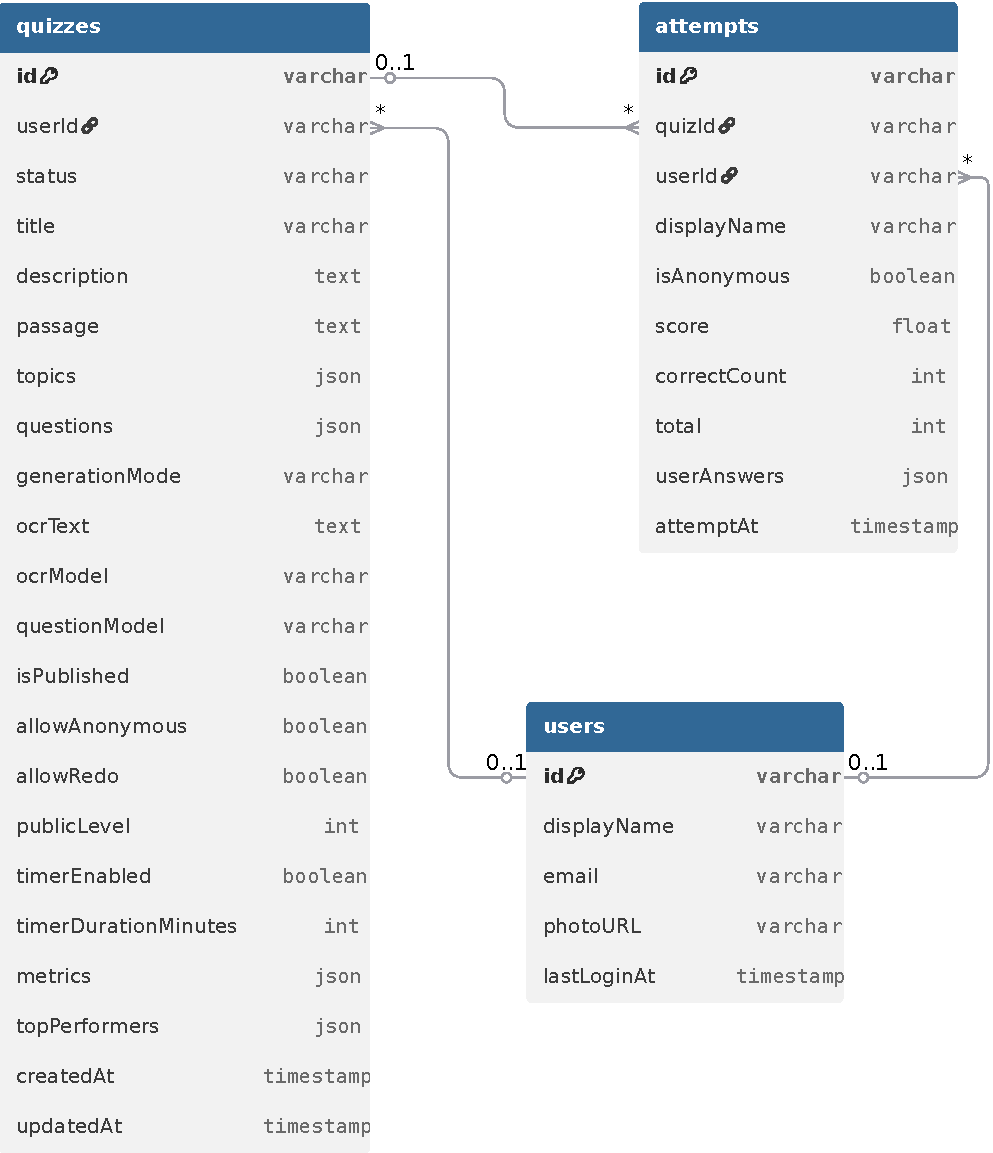
\includegraphics[width=\textwidth]{figures/database.pdf}
    \caption{Mô hình dữ liệu chính của Openlet gồm ba bảng: \textbf{users} (hồ sơ người dùng), \textbf{quizzes} (bài kiểm tra và câu hỏi), và \textbf{attempts} (lượt làm bài và kết quả)}
    \label{fig:openlet-data-model}
\end{figure}

Cloud Firestore được lựa chọn để lưu trữ vì bản chất dữ liệu của hệ thống Openlet có tính chất lồng nhau rõ rệt. Cụ thể, một bài kiểm tra không chỉ có các thông tin mô tả đơn giản mà còn chứa danh sách các câu hỏi, mỗi câu hỏi lại chứa nhiều lựa chọn khác nhau. Với đặc điểm dữ liệu như này, nếu sử dụng mô hình cơ sở dữ liệu quan hệ, hệ thống sẽ cần thực hiện nhiều lần kết hợp bảng thay vì chỉ cần một lần truy vấn như Firestore. \textbf{Bên cạnh đó, nền tảng còn hỗ trợ đồng bộ dữ liệu theo thời gian thực, rất phù hợp đối với những ứng dụng yêu cầu theo dõi tiến trình xử lý như Openlet.}

\section{Hiện thực các luồng chức năng cốt lõi}

Phần~\ref{sec:phan_tich_yeu_cau} đã phân tích và đưa ra các yêu cầu chức năng mà nền tảng làm bài kiểm tra trắc nghiệm trực tuyến hướng đến. Từ những thành phần hệ thống trong phần~\ref{sec:thiet-ke-he-thong}, khóa luận sẽ trình bày hiện thực hóa hai luồng chức năng chính tương ứng với hai tác nhân \textit{Giáo viên} và \textit{Học sinh}.

\subsection{Luồng tạo bài kiểm tra tự động}

Sơ đồ tuần tự cho chức năng tạo bài kiểm tra tự động được trình bày ở Hình~\ref{fig:sequence-create-quiz} để minh họa cách giao diện, nền tảng lưu trữ dữ liệu, nền tảng lưu trữ tệp, các hàm xử lý phía máy chủ và lớp mô hình trí tuệ nhân tạo phối hợp với nhau. Sơ đồ này làm rõ thứ tự xử lý từ lúc giáo viên tải tài liệu lên đến khi bài kiểm tra được cập nhật hoàn tất trên hệ thống..

\begin{figure}[htbp]
    \centering
    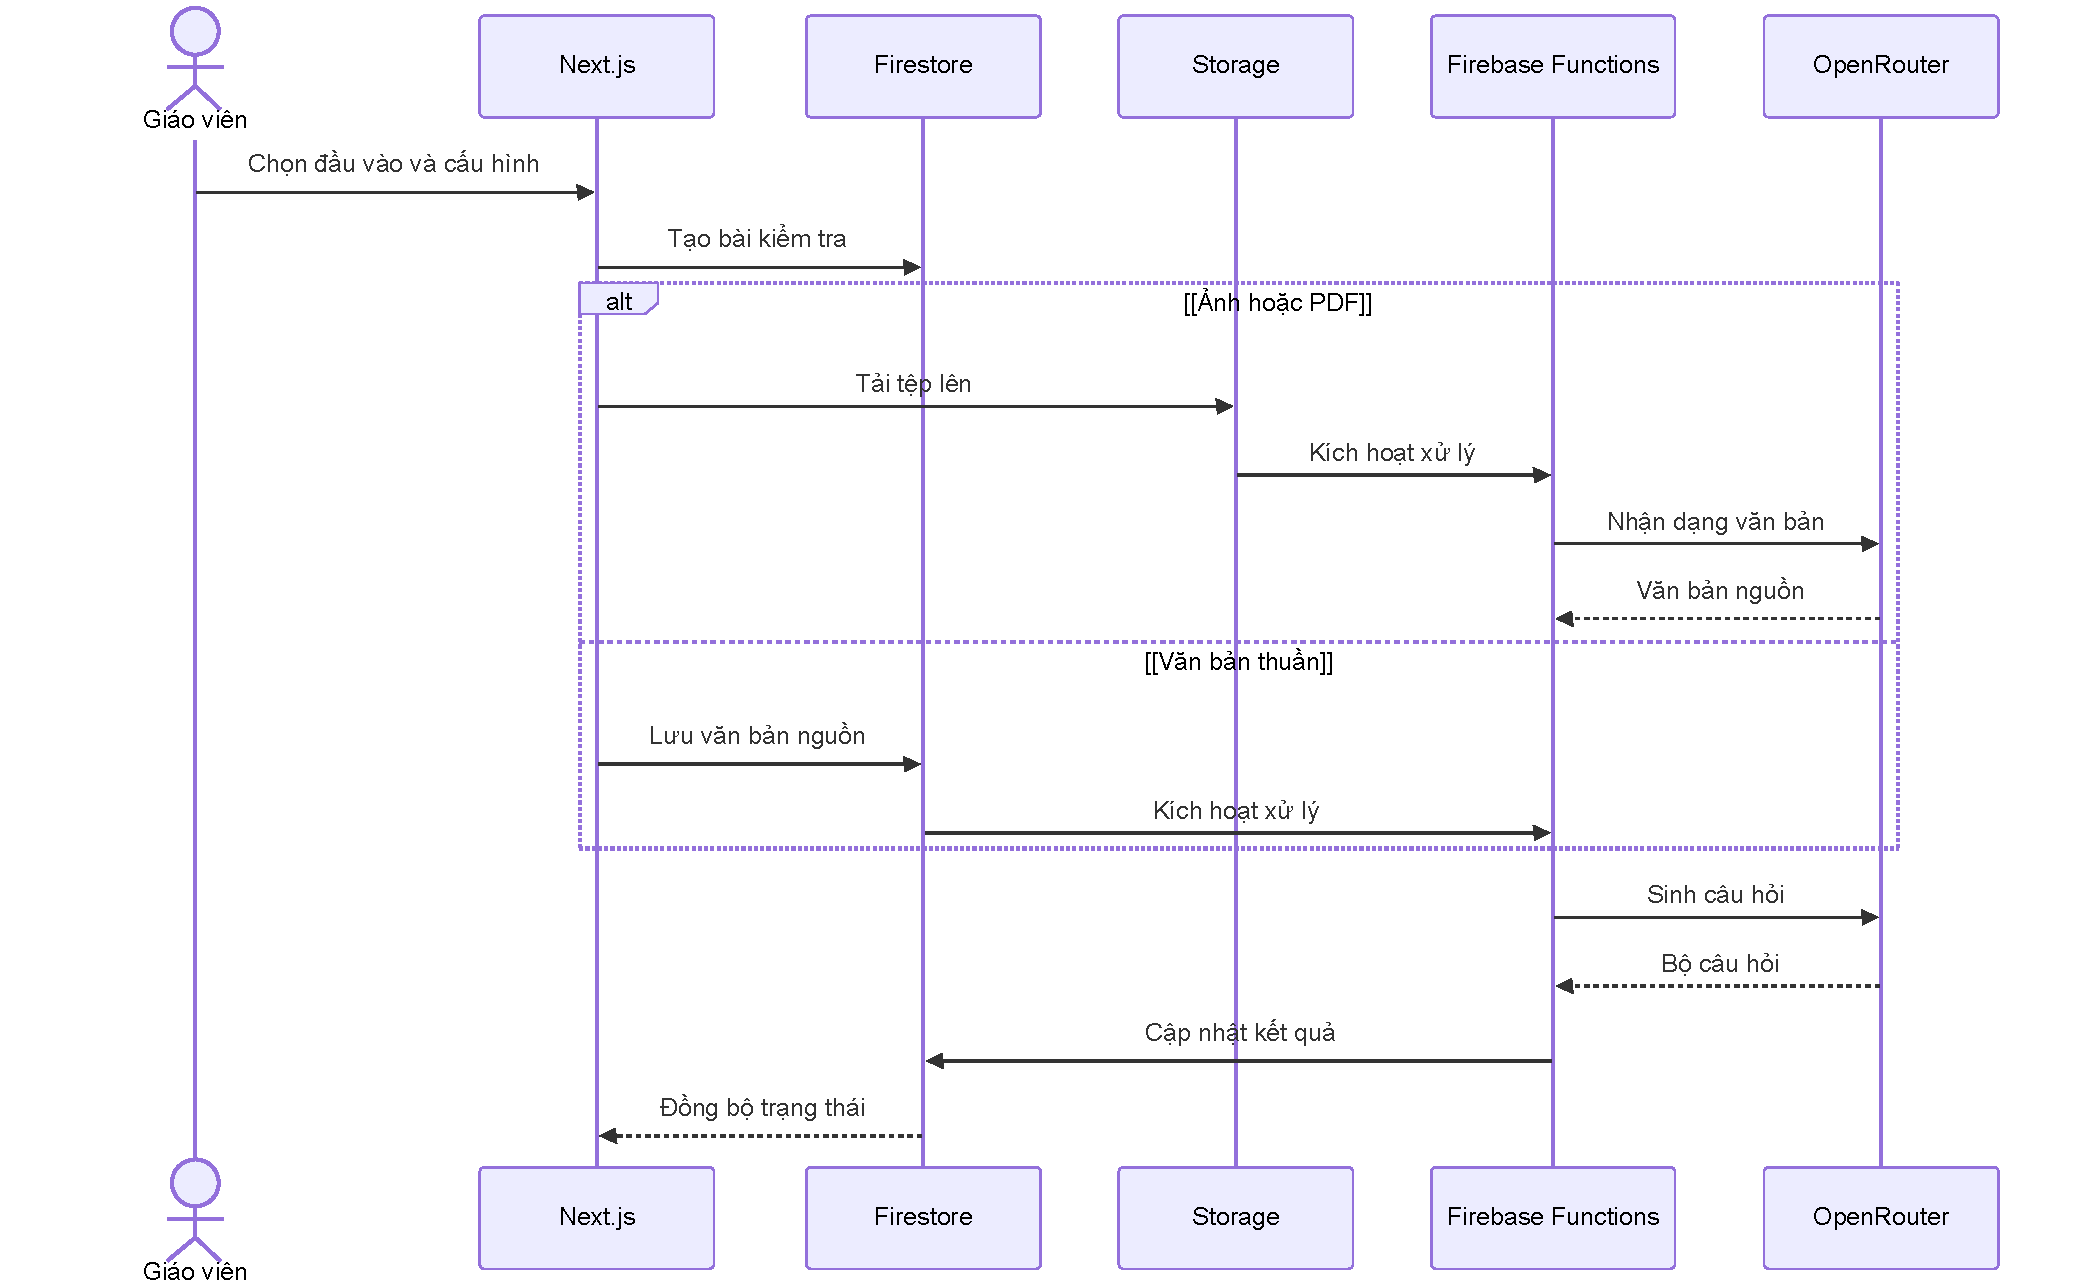
\includegraphics[width=0.95\linewidth]{figures/demo-sequence-quiz-creation.pdf}
    \caption{Biểu đồ tuần tự của luồng tạo bài kiểm tra tự động: từ tiếp nhận tài liệu đầu vào, qua OCR và MAS sinh câu hỏi, đến cập nhật trạng thái theo thời gian thực}
    \label{fig:sequence-create-quiz}
\end{figure}

Sau khi giáo viên tải tệp tài liệu văn bản lên, hệ thống sẽ khởi tạo một bản ghi để theo dõi tiến trình xử lý. Các Cloud Function sẽ được kích hoạt tuần tự: thực hiện OCR đối với ảnh hoặc tệp PDF, phân tích nội dung văn bản, sinh bài kiểm tra trắc nghiệm và cập nhật dữ liệu vào Firestore.

\subsection{Luồng truy cập, làm bài và nộp bài}

Sơ đồ tuần tự cho chức năng truy cập bài kiểm tra, làm bài và nộp bài được trình bày ở Hình~\ref{fig:sequence-play-submit} để làm rõ cách hệ thống bảo vệ đáp án đúng trong khi vẫn hỗ trợ chia sẻ công khai qua liên kết. Luồng này cũng cho thấy trách nhiệm chấm điểm được đặt ở phía máy chủ thay vì giao diện người dùng.

\begin{figure}[htbp]
    \centering
    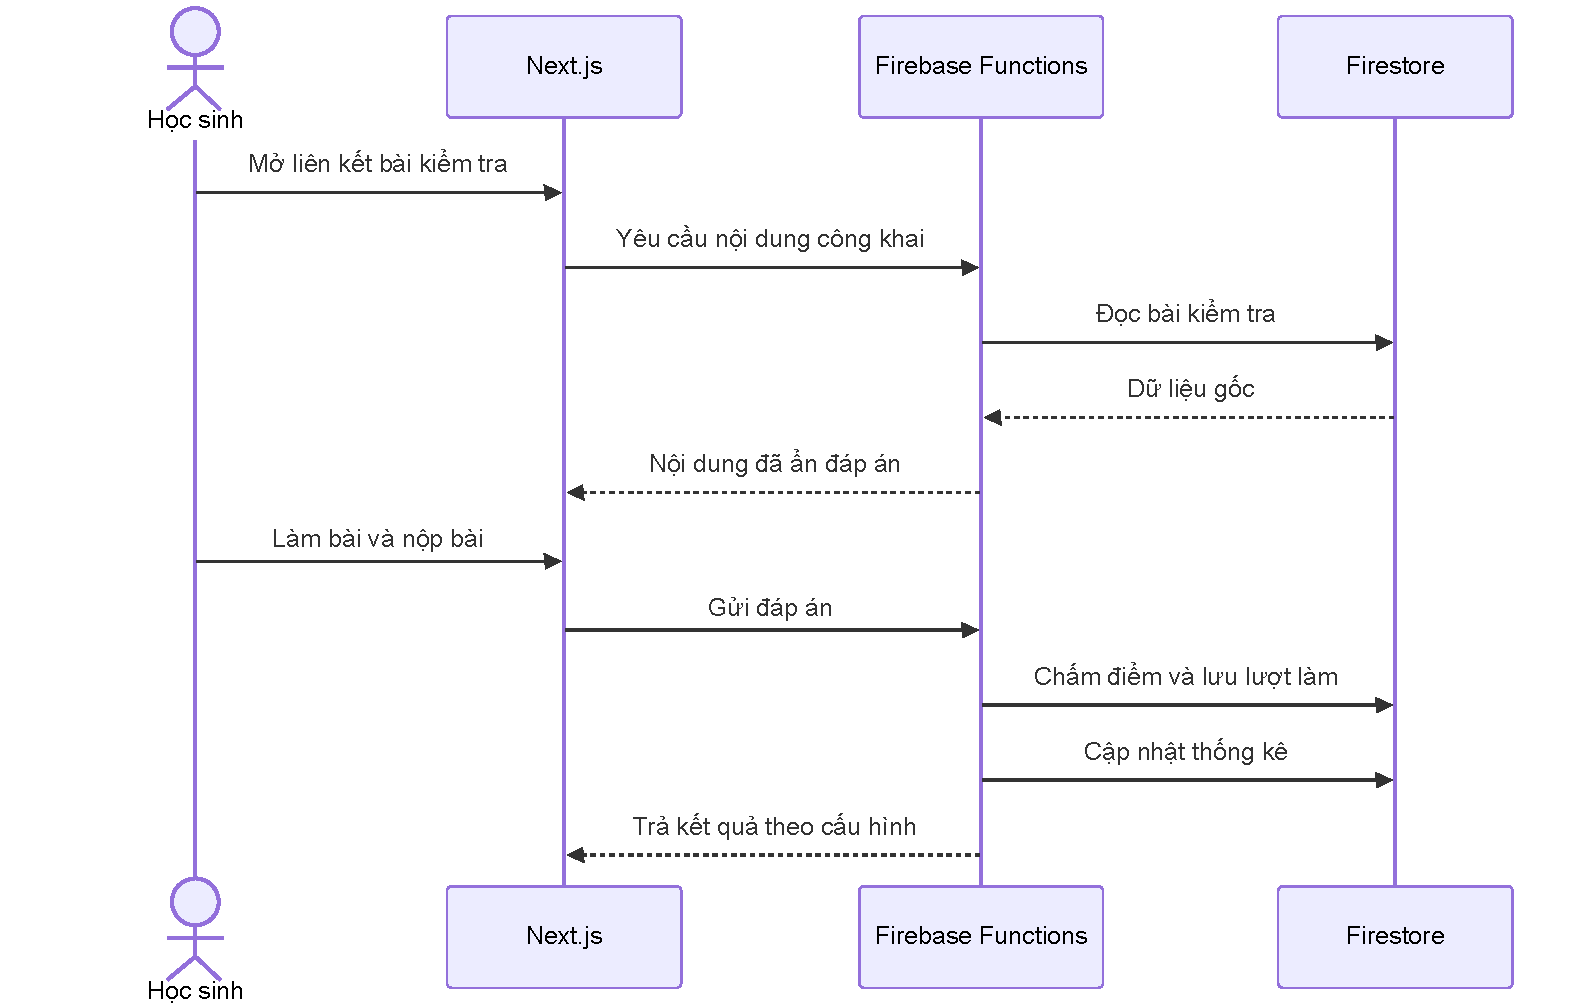
\includegraphics[width=0.95\linewidth]{figures/demo-sequence-quiz-play-and-submit.pdf}
    \caption{Biểu đồ tuần tự của luồng truy cập, làm bài và nộp bài: người làm bài nhận đề đã lọc đáp án, chấm điểm phía máy chủ, và nhận phản hồi theo mức cấu hình}
    \label{fig:sequence-play-submit}
\end{figure}

Học sinh tham gia bài kiểm tra bằng cách truy cập liên kết giáo viên chia sẻ. Sau đó, hệ thống yêu cầu nhập thông tin cá nhân hoặc đăng nhập với Google. Khi người dùng nộp bài, máy chủ chấm điểm, lưu lịch sử bài làm vào cơ sở dữ liệu. Cuối cùng hệ thống trả về điểm số kèm đáp án nếu giáo viên cấu hình cho phép.

\section{Giao diện tiêu biểu của ứng dụng}
\subsection{Giao diện dành cho giáo viên}

Giao diện quản trị của \textit{Giáo viên} được tổ chức liền mạch từ trang danh sách bài kiểm tra đến trang biên soạn bài kiểm tra. Trong môi trường biên soạn, giáo viên có thể chỉnh sửa câu hỏi, đáp án đúng hoặc tải tệp tài liệu để hệ thống chuyển thành các câu hỏi trắc nghiệm bằng kiến trúc đa tác tử đề xuất.

Hình~\ref{fig:ui-teacher-editor} minh họa màn hình biên tập trung tâm của giáo viên. Giáo viên nhìn thấy ngay kết quả sinh tự động, có thể sửa từng câu hỏi tại chỗ và không phải chuyển qua nhiều màn hình trung gian. Cách tổ chức này phù hợp với mục tiêu của ứng dụng là hỗ trợ giáo viên hoàn thiện nhanh một bài kiểm tra trước khi công bố.

\begin{figure}[htbp]
    \centering
    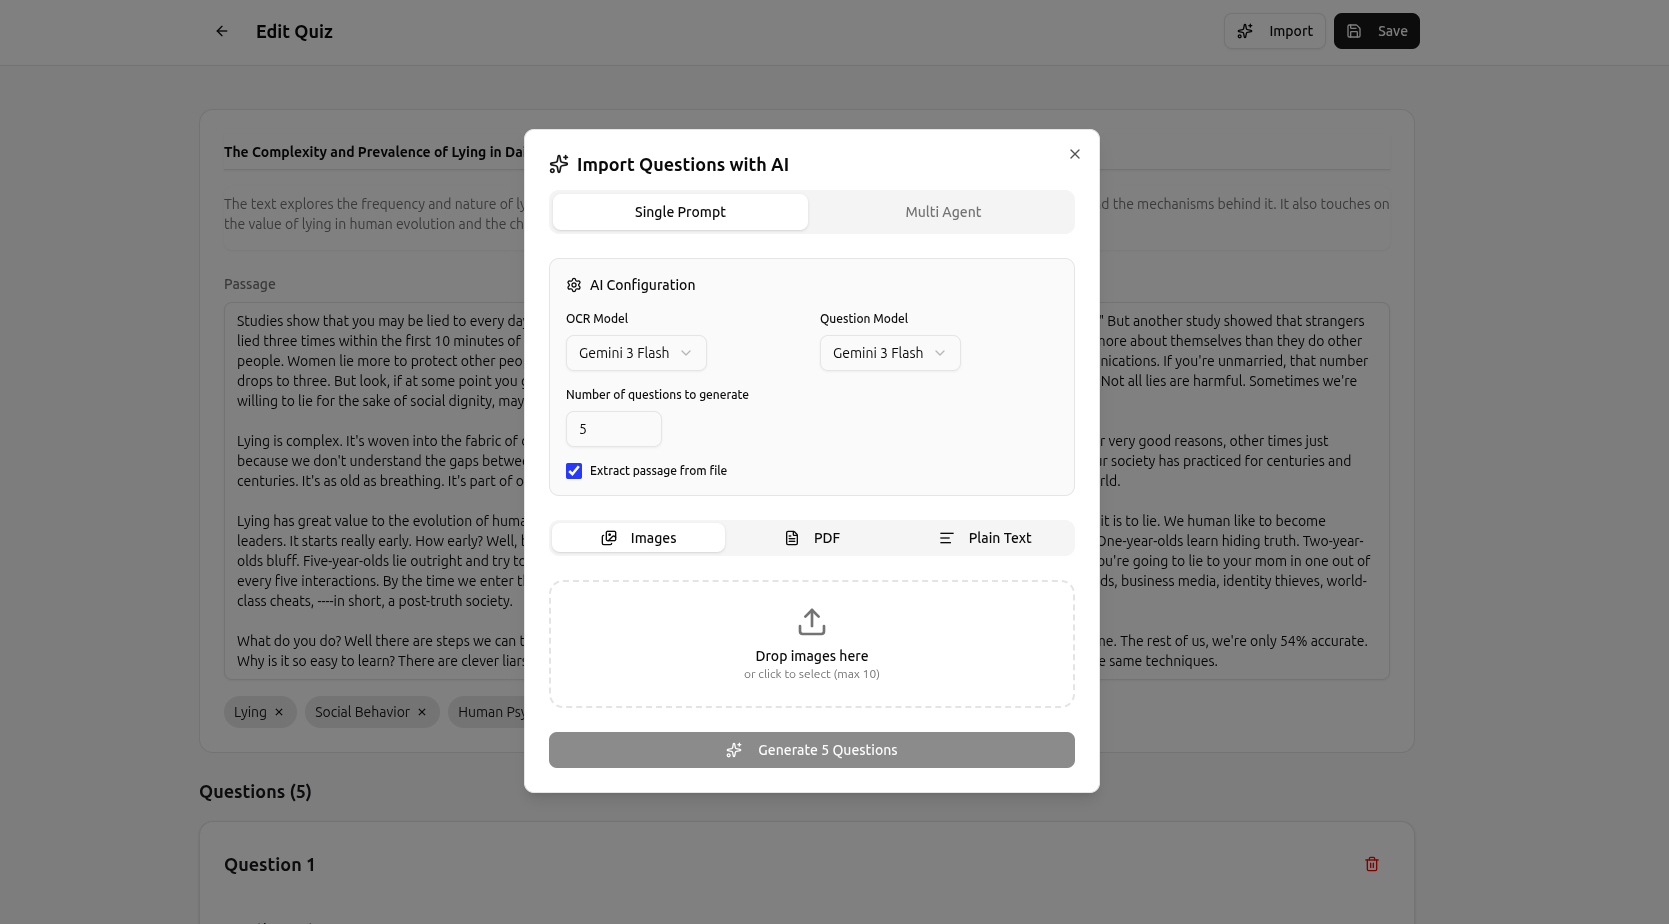
\includegraphics[width=0.95\linewidth]{figures/ui-edit.png}
    \caption{Giao diện biên tập bài kiểm tra dành cho giáo viên: hiển thị câu hỏi đã sinh tự động với các công cụ chỉnh sửa nội dung, phương án và cấp độ nhận thức}
    \label{fig:ui-teacher-editor}
\end{figure}

\subsection{Giao diện dành cho người làm bài}

Giao diện dành cho người làm bài được tối giản hơn đáng kể so với giao diện của giáo viên. Người học truy cập từ liên kết công khai, nhập tên hiển thị hoặc đăng nhập bằng tài khoản, sau đó được điều hướng tới màn hình làm bài. Trong quá trình làm bài, giao diện hiển thị rõ nội dung câu hỏi, các phương án, tiến độ làm bài và bộ đếm thời gian khi giáo viên bật tính năng này.

\begin{figure}[htbp]
    \centering
    \begin{minipage}{0.48\textwidth}
        \centering
        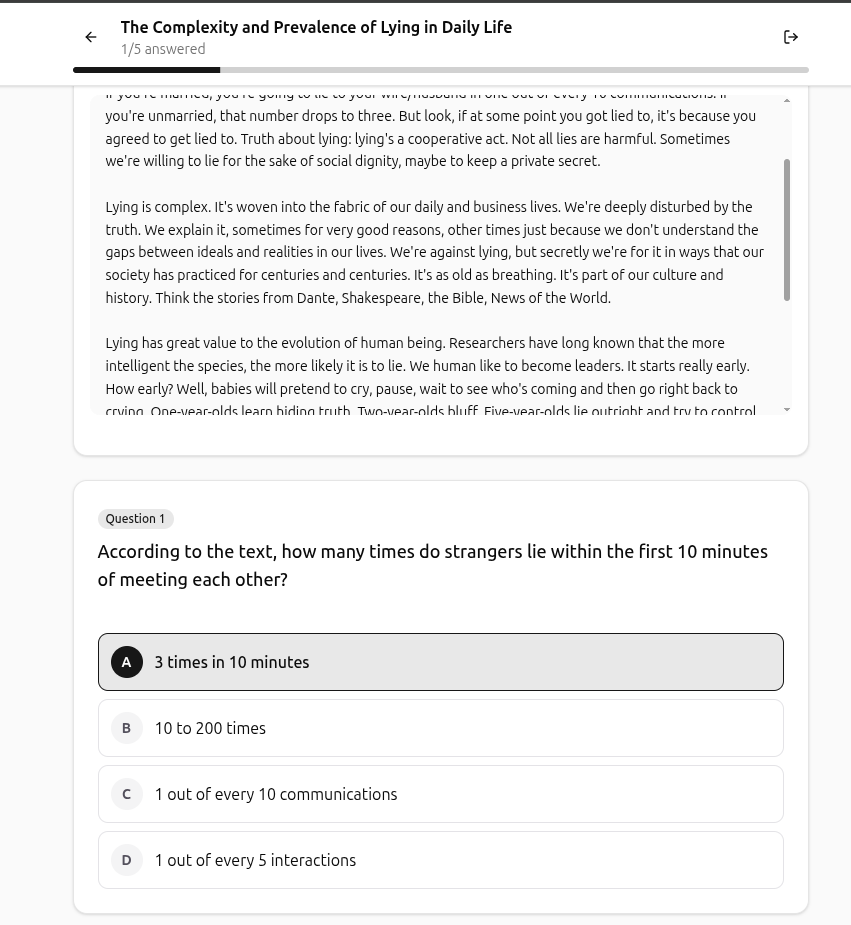
\includegraphics[width=\textwidth]{figures/ui-student-play.png}
    \end{minipage}
    \hfill
    \begin{minipage}{0.48\textwidth}
        \centering
        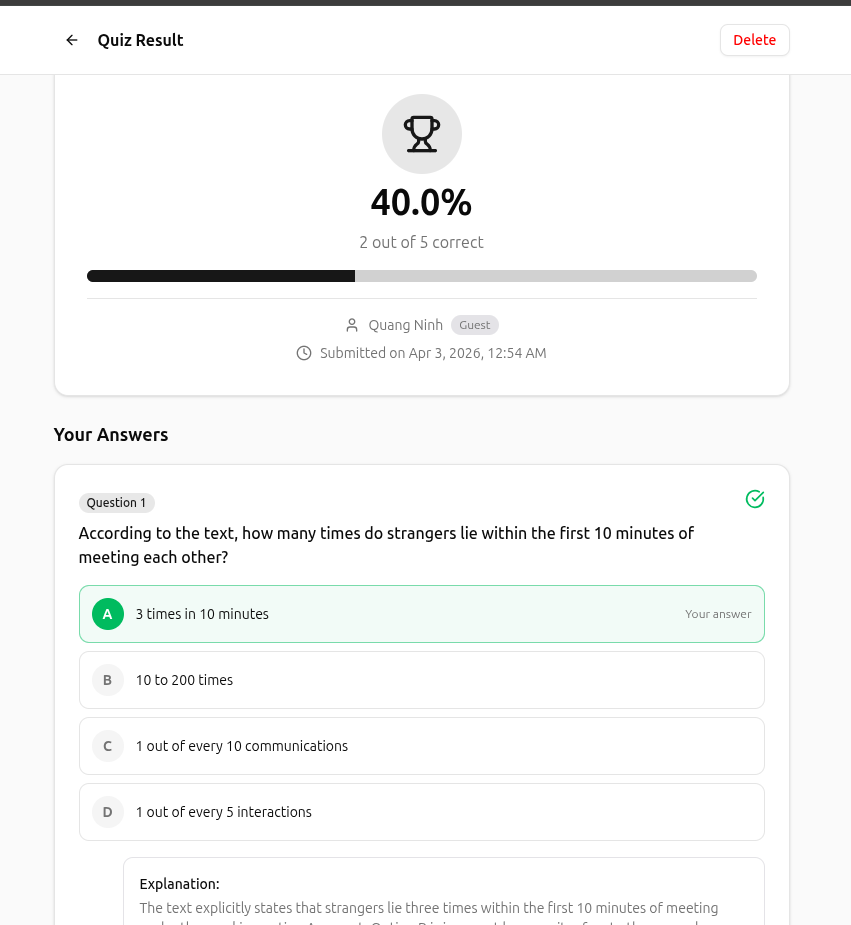
\includegraphics[width=\textwidth]{figures/ui-student-result.png}
    \end{minipage}
    \vspace{10pt}
    \caption{Giao diện làm bài (trái) và trang kết quả (phải): người làm bài chọn đáp án với bộ đếm thời gian, sau đó nhận phản hồi theo mức hiển thị cấu hình bởi giáo viên}
    \label{fig:ui-player-flow}
\end{figure}

Hình~\ref{fig:ui-player-flow} cho thấy cách Openlet tổ chức trải nghiệm của người làm bài theo hướng liền mạch. Màn hình làm bài ưu tiên khả năng tập trung và thao tác nhanh, trong khi màn hình kết quả ưu tiên tính rõ ràng của thông tin phản hồi. Sự phân tách này giúp người dùng không bị quá tải thông tin trong lúc làm bài, đồng thời vẫn nhận được mức hỗ trợ phù hợp sau khi hoàn thành.

\textbf{Nhìn chung, lớp giao diện của Openlet phản ánh đúng triết lý thiết kế của toàn hệ thống: giáo viên được cung cấp một không gian biên soạn và kiểm soát linh hoạt, còn người làm bài tiếp cận một trải nghiệm gọn, rõ và an toàn.} Đây là điều kiện cần để các kết quả nghiên cứu ở Chương~\ref{chap:phuong-phap} có thể được đưa vào sử dụng trong một ngữ cảnh nghiệp vụ thực tế.
